% Universidade Aberta
% Template TeX para relatório de trabalhos
% 2024
%
%
% Dados para a capa
\newcommand{\Titulo}{Diagramas de Componentes Git Activity Provider\\Padrões de Estrutura}
\newcommand{\Ano}{2024}
\newcommand{\Autor}{Hugo Gonçalves}
%
%
\documentclass[12pt,a4paper,final]{article}
\usepackage[stretch=10]{microtype}
\usepackage{csquotes}
\usepackage[portuguese]{babel}
\usepackage{polyglossia}
\setdefaultlanguage{portuguese}
\usepackage{graphicx}
\graphicspath{ {./images/} }
\usepackage[a4paper,top=3cm,bottom=3cm,left=3.5cm,right=2cm]{geometry}
\usepackage{booktabs}
\usepackage{newtxtext}
\usepackage{newtxmath}
\usepackage[pdfauthor=\Autor,
    pdftitle=\Titulo,
    colorlinks=true,
    linkcolor=black,
    citecolor=black,
    bookmarksopen=true]{hyperref}
\hypersetup{colorlinks, citecolor=black, urlcolor=black}
\usepackage{bookmark}
\usepackage{float}
\usepackage{tikz, tikz-uml}
\usepackage[style=apa, backend=biber, sortcites, url=true]{biblatex}
\addbibresource{ref.bib}
\renewcommand{\baselinestretch}{1.5}
\begin{document}
    \title{\Titulo}
    \author{\Autor}
    \date{\Ano}
    \pagenumbering{gobble}
    \begin{titlepage}
        \begin{center}
            \vspace*{4cm}

            \textbf{\large UNIVERSIDADE ABERTA}

            \textbf{\large UNIVERSIDADE DE TRÁS-OS-MONTES E ALTO DOURO}

            \vspace{1cm}

            \begin{minipage}{0.4\textwidth}
                \centering
                
\includegraphics[width=0.8\textwidth]{uab}
            \end{minipage}
            \begin{minipage}{0.4\textwidth}
                \centering
                
\includegraphics[width=0.8\textwidth]{utad}
            \end{minipage}

            \vspace{1.5cm}

            \textbf{\large \Titulo}

            \vspace{1.5cm}

            \textbf{\large \Autor}

            \vspace{2cm}

            \textbf{\large Mestrado em Engenharia Informática e Tecnologia Web}
            \vfill
            \textbf{\Ano}
        \end{center}
    \end{titlepage}
    \renewcommand{\contentsname}{Índice}
    \cleardoublepage
    \pagenumbering{roman}
    \tableofcontents
    \newpage
    \listoffigures
    \newpage
    \cleardoublepage
    \pagenumbering{arabic}


    \section{Introdução}\label{sec:introducao}
    O \textit{Git Activity Provider} utiliza o padrão de estrutura \textit{Adapter} em dois serviços distintos, o \textit{GitService} e o \textit{AnalyticsService}.
    De acordo com \cite{gamma_1994_design}, o padrão de estrutura \textit{Adapter}, converte interface de uma classe noutra interface que os clientes conhecem, permitindo que as classes sejam interoperáveis.
    O primeiro, adapta a interface pública do Github, combinando diversos \textit{endpoints} num modelo de dados único no AP, enquanto o segundo serviço, adapta o modelo de dados do AP e oferece a interface que a Inven!RA espera como definido por \cite{su15010857}, tal demonstra o diagrama de componentes representado na \autoref{fig:diagrama-componentes}.

    \begin{figure}[H]
        \centering
        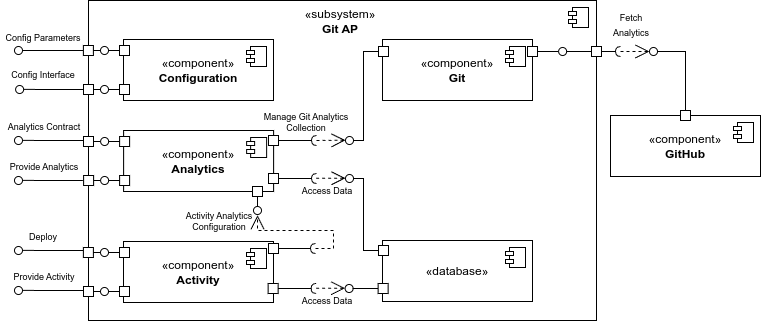
\includegraphics[width=0.9\textwidth]{diagrama_componentes_v2-AP.drawio}
        \caption{Diagrama de Componentes}
        \label{fig:diagrama-componentes}
    \end{figure}


    \section{Casos de uso}\label{sec:caso-de-uso}
    Tipicamente, os repositórios centralizados de \textit{git} oferecem uma API para aceder aos dados de repositórios.
    Estas APIs contém diversos \textit{endpoints} que as \textit{GitRepositoryStrategy} (\cite{gonalves_2024_gitrepositorystrategy}) utilizam para coletar as métricas oferecidas pelo \textit{Git Activity Provider}, seguindo assim a interface da API destes.

    \subsection{Git Service}\label{subsec:git-service}
    O \textit{Git Service} age como um \textit{Adapter} que adapta a interface das \textit{GitRepositoryStrategy}, a uma interface que o \textit{Analytics Service} conhece, criando, assim, baixo acoplamento entre o serviço de \textit{Analytics} e os repositórios \textit{git}.
    Esta adaptação, está representada a vermelho na chamada própria \textit{1. Create unique data model} no diagrama de sequência da \autoref{fig:diagrama-sequencia-coleta}.

    \subsection{Analytics Service}\label{subsec:analytic-sservice}
    O \textit{Analytics Service} age, também, como um \textit{Adapter}, ao transformar a interface do \textit{Git Service} na interface esperada pela Inven!RA.
    Além de adaptar a interface, processa também as métricas recolhidas e persiste-as na base de dados já no formato final a enviar para a Inven!RA. Este processamento acontece no caminho de escrita, como representado a vermelho na chamada própria \textit{2. Adapt GitAnalytics} no diagrama de sequência da \autoref{fig:diagrama-sequencia-coleta}, otimizando assim a latência da leitura.
    O processamento dos dados no caminho de escrita é abordado por \cite[Chapter 12, Observing Derived State]{kleppmann_2017_designing}.
    Esta otimização é vantajosa para os pedidos descritos pelo diagrama de sequência apresentado na \autoref{fig:diagrama-sequencia-obter} , onde obter métricas é uma simples \textit{query} à base de dados, uma vez que o \textit{Analytics Service}, persistiu os dados no formato em que serão lidos e retornados à Inven!RA.
    \begin{figure}[H]
        \centering
        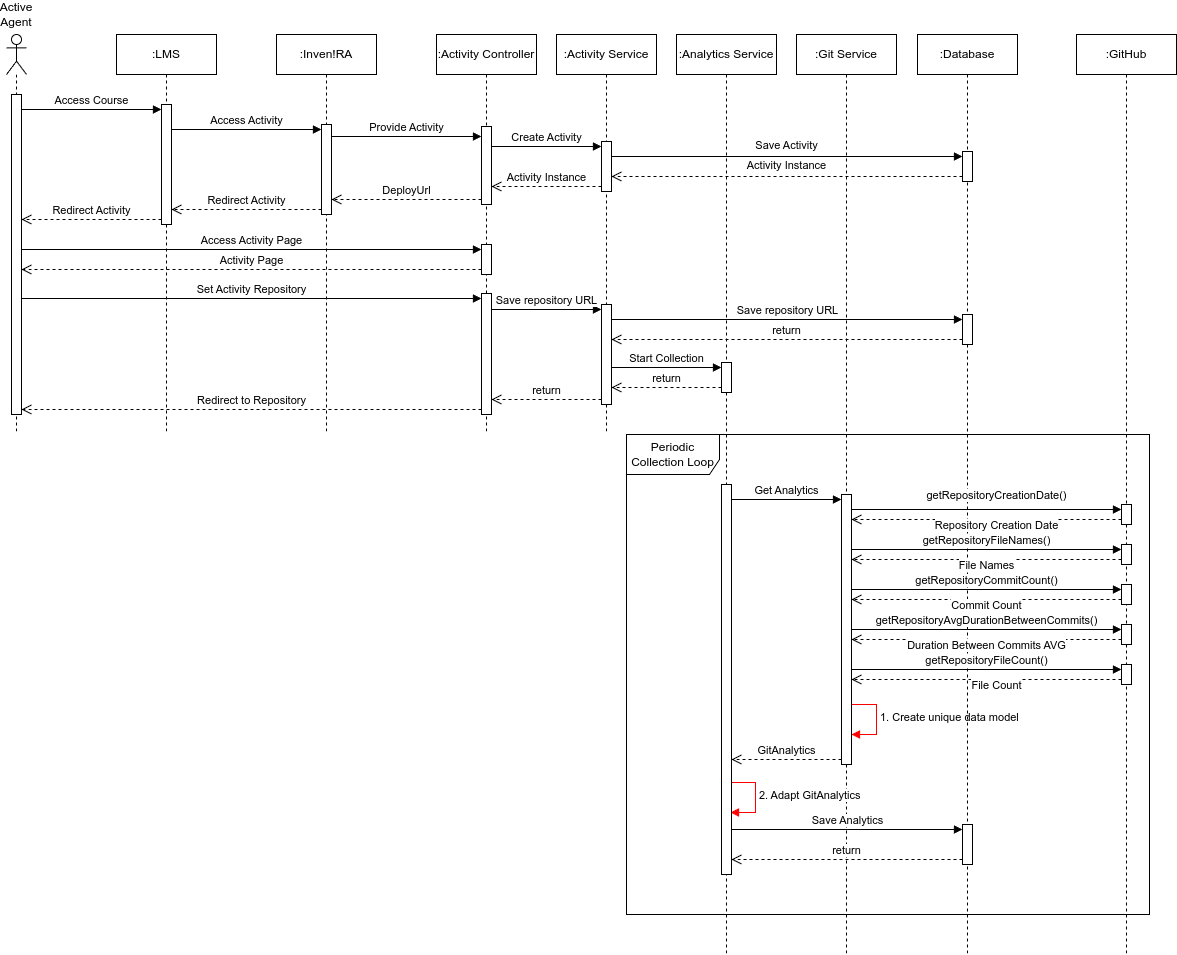
\includegraphics[width=0.9\textwidth]{diagramas_sequencia-uc1.drawio}
        \caption{Diagrama de Sequência - Inicio de coleta de métricas}
        \label{fig:diagrama-sequencia-coleta}
    \end{figure}

    \begin{figure}[H]
        \centering
        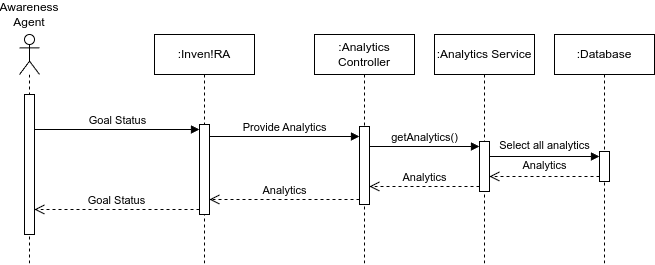
\includegraphics[width=0.9\textwidth]{diagramas_sequencia-uc2.drawio}
        \caption{Diagrama de Sequência - Obter métricas}
        \label{fig:diagrama-sequencia-obter}
    \end{figure}
    \newpage
    \printbibliography
\end{document}
